
En este capítulo abordaremos una de las preguntas centrales de la tesis: ¿puede ayudar el contexto a mejorar la performance de métodos automáticos de lenguaje de odio? Para intentar contestar esta pregunta, utilizaremos el dataset que construímos en el capítulo \ref{chap:dataset_creation}, y aplicaremos técnicas del estado del arte basadas en transformers. Exploraremos dos versiones de clasificadores: descontextualizadas, donde sólo observamos el comentario analizado; y contextualizadas, donde podemos consumir el título o el título y el cuerpo del artículo.

Proponemos en este capítulo dos tareas: detección ``plana'', donde sólo predecimos la característica de si hay o no discurso de odio; y la detección ``granular'', donde además predecimos todas las características ofendidas (potencialmente más de una). Analizaremos el impacto de agregar contexto para cada una de estos problemas de clasificación.


\section{Trabajos previos}
\label{sec:06_classification_previous}

Como contamos en la anterior sección, son pocos los trabajos y datasets que poseen contexto. Ver \ref{sec:dataset_previous} para un repaso de los distintos datasets contextualizados.

\citet{gao-huang-2017-detecting} propone dos tipos de modelos: regresiones logísticas y redes neuronales recurrentes. Para los modelos de regresiones logísticas, usan como inputs bolsas de palabras, bolsas de caracteres, vectores semánticos producidos con Linguistic Inquiry and Word Count (LIWC) \cite{pennebaker2001linguistic} y features de un lexicon de emociones \cite{mohammad2013nrc}. Por otro lado, utiliza LSTM bidireccionales con mecanismo de atención de Bahdanau \cite{bahdanau2014neural} usando embeddings \emph{word2Vec} de dimensión 100.

Un punto criticable de este trabajo es que utiliza el nombre de usuario como feature; algo que a priori no suele hacerse ya que permitiría ``prejuzgar'' a un usuario antes que por el contenido de sus tweets. Si bien es cierto que la información de usuarios y sus conexiones es valiosa, introducir esta información a nuestros modelos da lugar a posibles correlaciones espurias que es preferible evitar.


\begin{figure*}[t]
    \centering
    \begin{minipage}[b]{0.49\textwidth}
        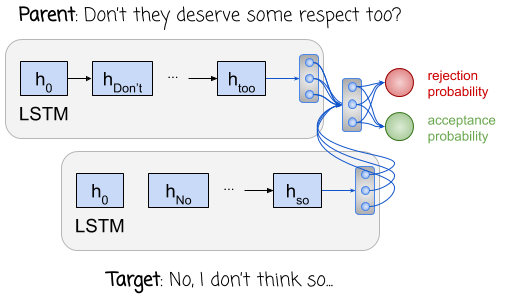
\includegraphics[width=\textwidth]{img/pavlopoulos_rnn_rnn_classifier.png}
    \end{minipage}
    \hfill
    \begin{minipage}[b]{0.49\textwidth}
        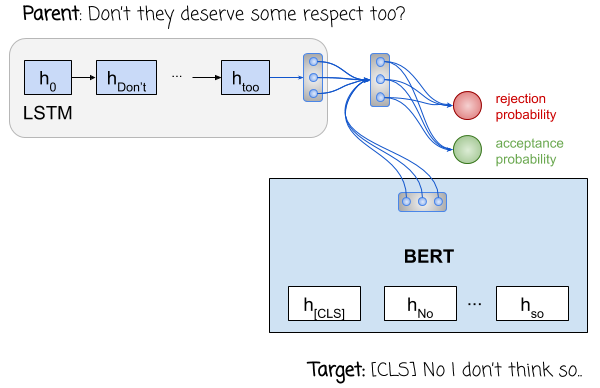
\includegraphics[width=\textwidth]{img/pavlopoulos_rnn_bert_classifier.png}
    \end{minipage}

    \begin{minipage}[b]{0.35\textwidth}
        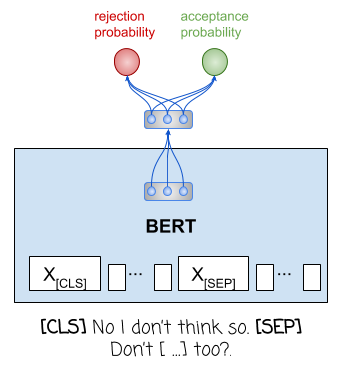
\includegraphics[width=\textwidth]{img/pavlopoulos_bert_sep_classifier.png}
    \end{minipage}


    \caption{Clasificadores que consumen contexto propuestos por \citet{pavlopoulos2020toxicity}. Los dos primeros clasificadores proponen una arquitectura de dos encoders, uno para el texto y otro para el contexto usando bi-LSTMs y BERT como posibilidades. El tercer clasificador propuesto es un BERT usando su estructura natural para codificar dos oraciones separadas por el token $SEP$ }
    \label{fig:pavlopoulos_classifiers}
\end{figure*}


En la sección \ref{sec:dataset_previous} hemos descripto el dataset construído por \citet{pavlopoulos2020toxicity}. Nos detendremos un momento para analizar sus experimentos de clasificación  ya que guardan importantes similaridades con lo que haremos en este capítulo. En ese trabajo se obtuvieron dos datasets de entrenamiento, uno etiquetado viendo el contexto y otro sin verlo. El dataset de test fue etiquetado viendo el contexto, considerando que el etiquetado es de mejor calidad usando más información. Tenemos entonces, dos preguntas: ¿mejora la performance de la tarea usando el dataset etiquetado con contexto? ¿mejora la performance del clasificador consumiendo información contextual? Estas dos preguntas nos brinda entonces dos elecciones: dataset de entrenamiento con o sin contexto, y clasificador con o sin contexto. Tenemos 4 posibles combinaciones de experimentos, sin aún considerar posibles técnicas de clasificación.

Para cada una de estas combinaciones, se consideraron técnicas del estado del arte de clasificación. Para aquellos clasificadores que no consumen contexto, las opciones son las mismas que hemos visto en capítulos anteriores: bi-LSTM o BERT. Para aquellos que sí consumen contexto, se evaluan dos estrategias: una, concatenar con algún caracter, y otra usando dos encoders distintos para el contexto y el texto. A su vez también utilizan la API Perspective de Google \todo{Agregar alguna cita de esto, y quizás alguna explicación en capítulo 4}.

Para todas las combinaciones posibles, si bien hay una mejora en la performance medida con ROC-AUC al usar contexto en ambas formas, esta no es significativa. De esto los autores concluyen que no pueden encontrar evidencia suficiente sobre la utilidad del contexto en la detección de toxicidad.

Algo a mencionar (que retomaremos en este y en el siguiente capítulo) es que usan dos versiones de BERT: una usando los pesos del modelo de BERT, y otro haciendo un ajuste de dominio () corriendo la tarea de MLM sobre un dataset grande y no etiquetado. En el caso de el trabajo mencionado, sólo hacen un fine-tuning sobre comentarios sueltos del dataset de Civil Comments. Esto podría tener algún efecto deteriorando la performance al usar contexto; sin embargo, en el BERT a secas (sin hacer ajustes) tampoco se observa mejora significativa en la performance.

Algunas limitaciones marcadas por los autores son:

\begin{itemize}
    \item Contexto muy pequeño: sólo el título más el comentario previo
    \item Se ignora el hilo completo de comentarios
    \item Los datos fueron sampleados aleatoriamente
\end{itemize}

En \citet{xenos-2021-context}, continuación de este trabajo, reetiquetaron el dataset de Civil Comments usando contexto y --como mencionamos en la sección \ref{sec:dataset_previous}-- presentaron una nueva tarea de detección de sensibilidad al contexto. Usando la API Perspective (y la estrategia de concatenación ``básica'' con algún caracter), notaron que la performance del clasificador que consume el contexto mejora con respecto al que no lo hace a medida que restringimos nuestra atención a comentarios más ``sensibles al contexto'' (de acuerdo a la métrica definida por los autores)


\section{Tareas de clasificación propuestas}



Ahora que tenemos este corpus especialmente diseñado que contiene el contexto, ahora dirigimos nuestra atención a responder nuestra pregunta original: ¿pueden los clasificadores aprovechar el contexto para mejorar su desempeño en la tarea de detección del discurso discriminatorio? Para ello, proponemos las siguientes tareas de clasificación:

\begin{enumerate}
    \item \textbf{Detección ``plain''}: Dado un tweet y su contexto, predecir si contiene contenido discriminatorio
    \item \textbf{Detección ``fine-grained''}: Dado un tweet y su contexto, predecir las características ofendidas (si hay alguna) y si contiene un llamado a la acción
\end{enumerate}


Puede pensarse la tarea de detección plana (la que usualmente se aborda en la literatura sobre el tema) como una relajación de la tarea detallada: mientras la primera sólo nos permite detectar si hay o no contenido discriminatorio, la segunda nos pide información más precisa acerca de las características ofendidas. Estas segunda tarea es posible dado que el dataset que construímos contiene esta información, algo usualmente faltante en otros datasets.

La tarea en su versión fine-grained nos permite a su vez tener mayor entendimiento de la salida e interpretar mejor sus errores, principalmente los falsos positivos. La figura \ref{fig:hate_detection_tasks} ilustra las dos tareas propuestas. Mientras en la tarea plana sólo debemos decidir la frontera entre si el contenido es discriminatorio o no, en la tarea fine-grained necesitamos decir en cuál de todas las intersecciones está el comentario y su contexto.

Planteándolos como problemas de clasificación, la detección plana consta de predecir una sola etiqueta binaria, mientras que la tarea fine-grained consta de $n$ etiquetas binarias; es decir, $n$ problemas distintos de clasificación. Vale mencionar que, entendiendo una tarea como una relajación de la otra, si tenemos un clasificador entrenado para la tarea fine-grained podemos construir un clasificador para la tarea plana tomando la disyunción lógica de sus salidas. Retomaremos esta idea más adelante al hablar de cómo evaluamos nuestras técnicas de clasificación para cada tarea.

%%
%%
%% Link
%% https://docs.google.com/drawings/d/11sAaOuGJlU0P61mkrPxKduFwnNOuPV31tXUFJWEwbVU/edit?usp=drive_web&ouid=117313784631536396179
%%
%%

\begin{figure}[t]
    \centering
    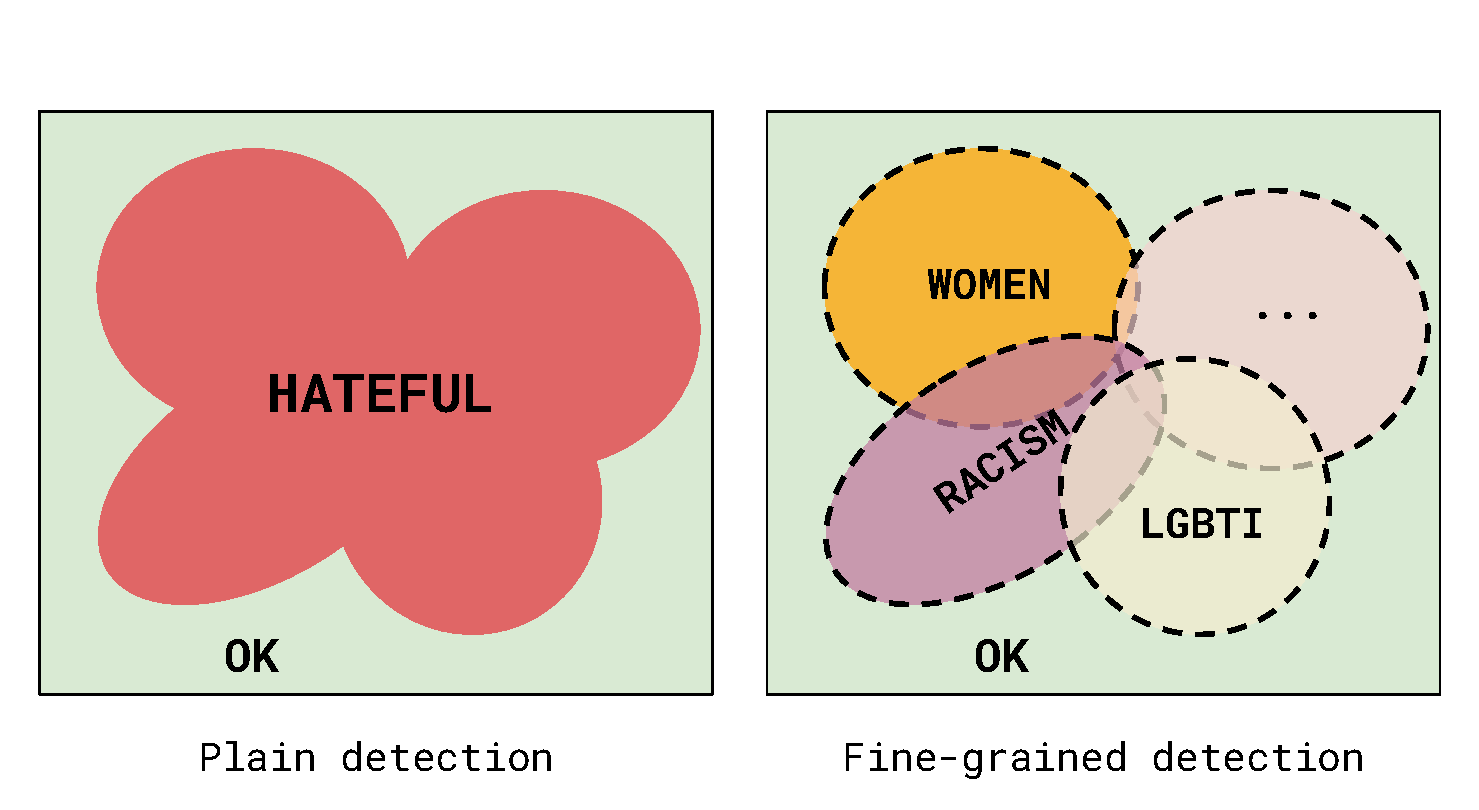
\includegraphics[width=\textwidth]{img/hate_detection_tasks.pdf}
    \caption{Tareas propuestas de detección}
    \label{fig:hate_detection_tasks}
\end{figure}

To test our hypothesis, for each task we trained classifiers having as input the following comibinations:

\begin{enumerate}
    \item The comment
    \item The title and the comment
    \item The title, the body and the comment
\end{enumerate}


\subsection{Cotas a la performance}

\begin{table}
    \centering
    \begin{tabular}{lll|ll}
        \hline
                   & \multicolumn{2}{c}{Entre anotadores} & \multicolumn{2}{c}{Contra gold} \\
        {}         &  F1 mean&  F1 median  & F1 Mean  &  F1 Median \\
        \hline
        HATEFUL    &  0.6525 &   0.6751    & 0.8285   &   0.8515   \\
        CALLS      &  0.6042 &   0.7037    & 0.7741   &   0.9148   \\
        WOMEN      &  0.7258 &   0.7368    & 0.8371   &   0.8275   \\
        LGBTI      &  0.8939 &   0.9600    & 0.9660   &   0.9743   \\
        RACISM     &  0.9458 &   0.9592    & 0.9667   &   0.9731   \\
        CLASS      &  0.7310 &   0.7500    & 0.8058   &   0.8391   \\
        POLITICS   &  0.7370 &   0.7777    & 0.8920   &   0.9189   \\
        DISABLED   &  0.7973 &   0.8800    & 0.8976   &   0.9392   \\
        APPEARANCE &  0.8033 &   0.9024    & 0.9026   &   0.9493   \\
        CRIMINAL   &  0.8180 &   0.9473    & 0.9614   &   0.9788   \\
        \hline
    \end{tabular}
    \caption{Estadísticos de los cálculos de F1 entre anotadores - modo jerárquico}
    \label{tab:ia_f1_scores}
\end{table}

Como observamos en la anterior sección, la tarea de detección de lenguaje discriminatorio contiene una alta cantidad de ruido, y el acuerdo entre humanos es moderado. En este contexto, cabe preguntarse cuál es la máxima performance que puede lograr un clasificador para esta tarea. Por la misma naturaleza del problema, claramente no puede ser perfecta.

Para obtener algunas medidas de esto, calculamos en primer lugar las F1 usando todos los posibles pares de anotadores. Como la F1 es simétrica (invirtiendo roles se invierten la precisión y la sensibilidad) no necesitamos hacer ninguna asunción sobre cuál sus roles.

Algo a tener en cuenta es que nuestra métrica final será contra la etiqueta resultante del (nuestro \emph{gold standard}). Una cota que seguro está por arriba de nuestra performance es el acuerdo que haya entre los anotadores y este \emph{gold standard}; hay que también observar que cada etiqueta ``de oro'' codifica información de sus anotaciones, con lo cual éste número es una cota superior sin dudas pero también pueden ser demasiado ``gruesa''.

La tabla \ref{tab:ia_f1_scores} contiene estadísticos de estos cálculos, tanto entre anotadores como contra el \emph{gold-standard}. Como podemos observar, la mediana entre anotadores de la F1 (usada para obviar outliers) es relativamente baja para la detección de odio ($\sim 0.67$), mientras que contra el gold standard es de $0.85$. De esto entendemos que la performance máxima en la detección está entre esos dos números.

Por otro lado, para el resto de las características observamos números más elevados, pero hay que recordar que estos cálculos están hecho \textbf{solamente} entre tweets etiquetados como odiosos. Si obviamos esta restricción (lo que llamamos ``modo libre''), la performance esperada baja sustancialmente. La tabla \ref{tab:ia_f1_scores_free_mode} muestra estos números, tanto calculado entre anotadores como contra el \emph{gold standard}.

\begin{table}
    \centering
    \begin{tabular}{lll|ll}
        \hline
                   & \multicolumn{2}{c}{Entre anotadores} & \multicolumn{2}{c}{Contra gold} \\
        {}         &  F1 mean&  F1 median  & F1 Mean  &  F1 Median \\
        \hline
        CALLS      &  0.4341 &   0.4950   &  0.7042   &   0.8424  \\
        WOMEN      &  0.4896 &   0.4676   &  0.7406   &   0.7593  \\
        LGBTI      &  0.5959 &   0.5765   &  0.8462   &   0.9152  \\
        RACISM     &  0.6532 &   0.6444   &  0.8712   &   0.8789  \\
        CLASS      &  0.4431 &   0.4444   &  0.7220   &   0.7317  \\
        POLITICS   &  0.4609 &   0.4360   &  0.7951   &   0.8155  \\
        DISABLED   &  0.5502 &   0.6000   &  0.8127   &   0.8421  \\
        APPEARANCE &  0.6485 &   0.7428   &  0.8314   &   0.9146  \\
        CRIMINAL   &  0.5265 &   0.5801   &  0.8415   &   0.9292  \\
        \bottomrule
    \end{tabular}

    \caption{Estadísticos de los cálculos de F1 entre anotadores - modo libre. Cada característica es tomada como una etiqueta binaria independientemente del cálculo de odio}
    \label{tab:ia_f1_scores_free_mode}
\end{table}


\subsection{Preprocessing}

Para cada tweet, aplicamos el siguiente procesamiento previo: primero, cortamos las repeticiones de caracteres hasta tres ocurrencias; risas normalizadas; los identificadores de usuario (\emph{@user}) se reemplazan por un token especial \emph{[USER]}; convertimos emojis en una representación de texto usando la biblioteca de python \emph{emoji} \footnote {\url{https://github.com/carpedm20/emoji/}}. Los hashtags se eliminan, están rodeados por una ficha especial \emph{[HASHTAG]} y se dividen en palabras si están en mayúsculas.

Aunque no realizamos un análisis de ablación para evaluar el impacto de cada paso del preprocesamiento, el proceso general pareció mejorar el rendimiento de la clasificación en el conjunto de datos de desarrollo.

\subsection{Clasificadores}
\label{sec:contextualized_classifiers}

%%
%%
%% Link a Draw
%% https://docs.google.com/drawings/d/1F8iVSIRqHhGkQ0zglxqXLGD36RHZ9OhHMZYsg_xFOS4/edit
%%
%%

\begin{figure}
    \centering
    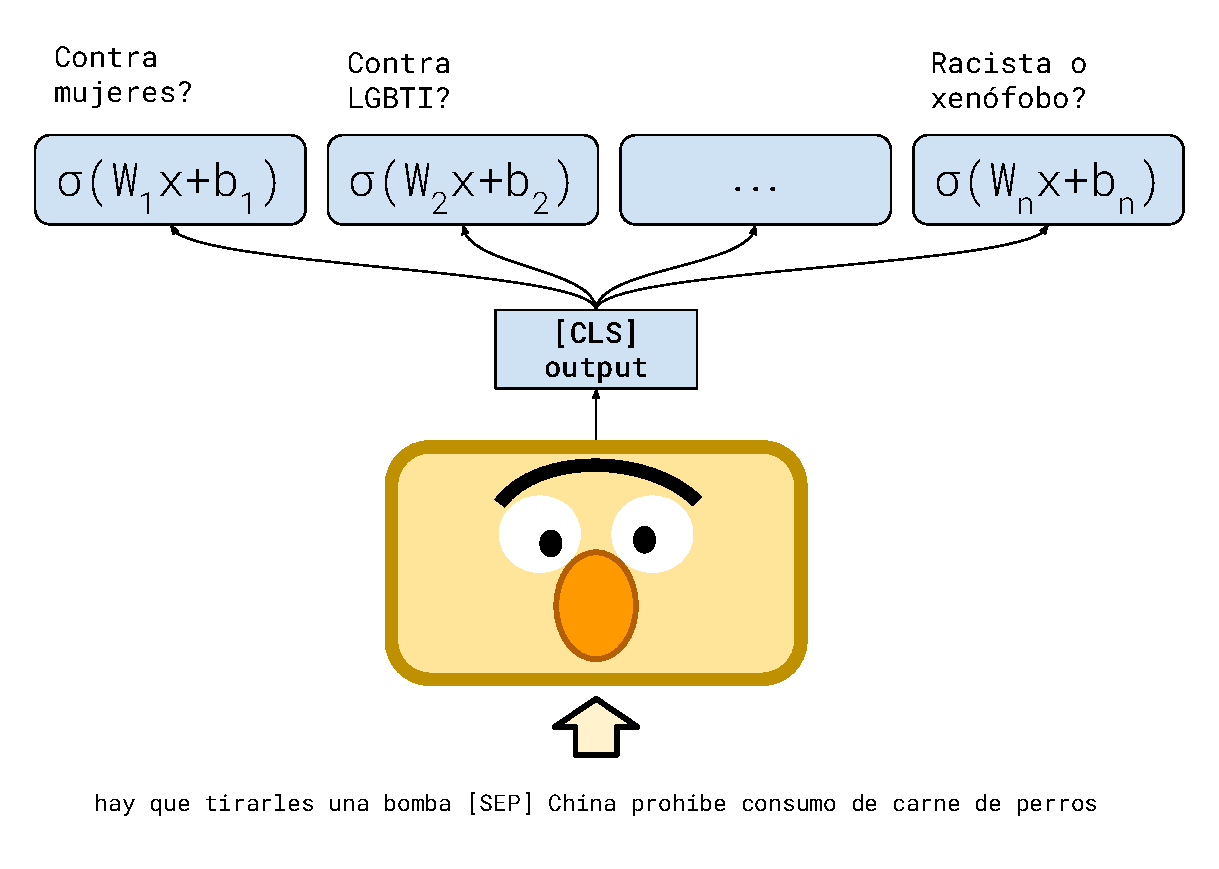
\includegraphics[width=\textwidth]{img/bert_multioutput.pdf}
    \caption{Muestra de la recolección de datos}
    \label{fig:bert_classifier}
\end{figure}


Los clasificadores propuestos se basan en \emph{BETO}\cite{canete2020spanish}, una versión en español de \emph{BERT} \cite{devlin2018bert}; para más referencias sobre BERT ver sección XXX.

Para la tarea de detección del discurso de odio, presentamos versiones sin contexto y conscientes del contexto, utilizando el título y el cuerpo completo como posibles contextos. Usamos el token especial BERT \emph {[SEP]} para codificar el contexto y el texto analizado. Recuerde que el token \emph {[SEP]} se usa para la tarea de predicción de la siguiente oración (tarea NSP) en el preentrenamiento al estilo BERT.

En cuanto a la detección de características ofendidas, consideramos este problema como una tarea de clasificación multibinaria; es decir, dado un texto odioso y una característica protegida, lo consideramos como una tarea de clasificación binaria para predecir si el texto ofende la característica respectiva. En lugar de entrenar un clasificador diferente para cada característica, entrenamos un BERT de múltiples salidas, compartiendo todos sus pesos con la excepción de 9 capas lineales diferentes para cada salida. La pérdida utilizada es

\begin{equation*}
    J = \sum\limits_{c \in CHAR \cup \{CALLS\}} J_c
\end{equation*}

donde $CHAR$ es el conjunto de todas las características protegidas (MUJERES, LGBTI, RACISMO, CLASE, etc.) y $CALLS$ es `` llamadas a la acción ''. $ J_c $, ya que cualquier $ c $ es una pérdida de entropía cruzada binaria.

Para tener costos computacionales más amigables, limitamos nuestras secuencias a 128, 256 y 512 tokens para el modelo no contextualizado, el modelo de título y el modelo de título y cuerpo, respectivamente.

Una práctica cada vez más extendida en trabajos del área de clasificación de documentos es realizar una adaptación de dominio sobre textos relacionados a nuestro problema; en nuestro caso, al dominio de redes sociales. Esto se realiza corriendo la tarea de MLM (ver sección YYY) sobre un dataset grande y no supervisado relacionado a nuestro dominio, o directamente sobre el dataset de la tarea si esto no está disponible. En la sección \ref{sec:domain_adaptation_previous_work} del siguiente capítulo haremos una reseña de esta técnica, pero por lo pronto podemos entender que ajusta nuestro ``conocimiento'' a los textos disponibles (en este caso, BETO entrenado en Wikipedia y noticias es ajustado a un dominio de tweets).

Para lo que nos concierne en esta sección, \citet{pavlopoulos2020toxicity} realizó una adaptación de dominio sobre los comentarios del corpus de \emph{Civil Comments} (a lo que denomina BERT-CCTK), sin realizar una adaptación sobre textos con contexto. Proponemos, entonces, y a diferencia de este trabajo que tomamos como referencia, 3 tipos de adaptaciones: una adaptación sin contexto, una adaptación con el contexto del tweet, y una adaptación con el contexto del tweet y el cuerpo de la noticia.
\todo{agregar secciones}

Realizamos el ajuste utilizando el sobrante de la recolección de datos del anterior capítulo: alrededor de 288k artículos y 5.1M comentarios\footnote{Utilizamos algunos datos extra recolectados a posteriori de lo mencionado en el capítulo anterior}. La tabla \ref{tab:hs_ft_hyperparameter} contiene los hiperparámetros utilizados. Para correr estos experimentos, las corrimos sobre una TPU v2-8 y una máquina de Google Colab Pro por alrededor de 10 hs (en su largo de cadena máximo).

\begin{table}[t]
    \centering
    \begin{tabular}{ll}
        \toprule
        Hiperparámetro & Valor         \\
        \midrule
        Steps          & $10K$           \\
        Batch size     & 2048            \\
        max seq length & 128, 256 y 512  \\
        $\beta_1$      & $0.9$           \\
        $\beta_2$      & $0.98$          \\
        $\epsilon$     & $10^{-6}$       \\
        decay          & $0.01$          \\
        Peak LR        & $4*10^{-4}$     \\
        warmup ratio   & 0.1             \\
        \bottomrule
    \end{tabular}
    \caption{Hiperparámetros para la adaptación de dominio de BERT}
    \label{tab:hs_ft_hyperparameter}
\end{table}


\section{Resultados}


\begin{table*}[ht!]
    \centering
    \begin{tabular}{lllll}
        \toprule
        Model &          Precision &             Recall &                 F1 &           Macro F1 \\
        \midrule
        BERT No Context &  $0.682 \pm 0.020$ &  $0.593 \pm 0.018$ &  $0.634 \pm 0.006$ &  $0.785 \pm 0.003$ \\
        BERT Title      &  $0.751 \pm 0.012$ &  $0.603 \pm 0.011$ &  $0.669 \pm 0.007$ &  $0.807 \pm 0.004$ \\
        BERT Title+Body &  $0.738 \pm 0.008$ &  $0.616 \pm 0.005$ &  $0.671 \pm 0.004$ &  $0.808 \pm 0.002$ \\
        \bottomrule
    \end{tabular}


    \caption{Task A: Hate speech detection classification results. Each row contains the performance of the models in complexity order: from the model having no context to the model having full context (title and body). }
    \label{tab:task_a_results}
\end{table*}


La tabla \ref{tab:task_a_results} contiene los resultados de la clasificación, medidos por precisión, recall, F1 de la clase positiva y Macro F1 entre las dos clases. Podemos observar que agregar contextos parece mejorar el desempeño; en particular, agregar el texto parece proporcionar suficiente contexto para la tarea de detección del discurso de odio. Agregar el cuerpo mejora marginalmente el rendimiento, pero a un costo computacional más alto (recuerde que la longitud máxima con título se establece en 256, y en el otro caso es 512). La mejora en la puntuación de F1 con solo agregar el título es de aproximadamente 3 puntos; título y cuerpo suma alrededor de 3,5 puntos F1 sobre la clasificación no contextualizada. Al analizar los modelos contextuales, el cuerpo completo parece mejorar el recuerdo al tiempo que disminuye ligeramente la precisión, con una puntuación general igual de F1 que el modelo de solo título.

\begin{table*}
    \centering
    \begin{tabular}{lrrrrrr}
        \toprule
        Métrica        &\mc{2}{Sin Contexto}& \mc{2}{Tweet}          &  \mc{2}{Tweet + Cuerpo}    \\
        \hline
        Calls F1       & 0.646 &    0.651   & 0.638 &\textbf{0.685}  & 0.653 &    0.680    \\
        Women F1       & 0.373 &    0.389   & 0.411 &\textbf{0.421}  & 0.381 &\textbf{0.421} \\
        Lgbti F1       & 0.351 &    0.366   & 0.451 &\textbf{0.482}  & 0.427 &    0.445    \\
        Racism F1      & 0.635 &    0.653   & 0.688 &\textbf{0.720}  & 0.691 &    0.711    \\
        Class F1       & 0.401 &    0.433   & 0.491 &\textbf{0.511}  & 0.451 &    0.476    \\
        Politics F1    & 0.555 &    0.611   & 0.579 &0.625           & 0.591 &\textbf{0.648} \\
        Disabled F1    & 0.551 &    0.582   & 0.585 &\textbf{0.609}  & 0.557 &    0.578    \\
        Appearance F1  & 0.726 &    0.742   & 0.741 &\textbf{0.766}  & 0.755 &    0.758    \\
        Criminal F1    & 0.513 &    0.529   & 0.650 &\textbf{0.699}  & 0.654 &    0.668    \\
        \hline
        Macro F1       & 0.528 &    0.551   & 0.582 &\textbf{0.613}  & 0.573 &    0.598    \\
        Macro Precision& 0.558 &    0.630   & 0.642 &\textbf{0.702}  & 0.677 &    0.678    \\
        Macro Recall   & 0.506 &    0.499   & 0.540 &\textbf{0.551}  & 0.504 &    0.541    \\
        \hline
        Hate Precision & 0.679 &    0.712   & 0.722 &\textbf{0.760}  & 0.748 &    0.741    \\
        Hate Recall    & 0.621 &    0.631   & 0.642 &\textbf{0.666}  & 0.621 &    0.658    \\
        Hate F1        & 0.648 &    0.668   & 0.679 &\textbf{0.710}  & 0.679 &    0.697    \\
        \bottomrule
        \end{tabular}
    \caption{Performance de los modelos para la tarea de detección fina de discurso de odio. Cada modelo es un BERT con 3 posibles entradas: sólo el comentario (\emph{Sin contexto}), el tweet de la noticia a la cual responde el comentario (\emph{Tweet}), y el tweet más el cuerpo de la noticia (\emph{Tweet + Cuerpo}). Para cada una de estas posibilidades usamos dos versiones: una sobre BETO y otra sobre BETO ajustado al dominio (FT) de acuerdo a lo descripto en la sección \ref{sec:contextualized_classifiers}. Reportamos también la F1 sobre la clase de discurso de odio, ignorando las características de la misma manera que hacemos en la detección plana}
    \label{tab:task_b_results}
\end{table*}



La tabla \ref{tab:task_b_results} muestra los resultados de los experimentos de clasificación para la tarea de detección fina, medida en F1 para cada una de las características, y las medidas agrupadas de forma macro precision, recall, y F1. Se muestra en cada caso el resultado de la media de 10 corridas del experimento. Como era esperable, la ganancia de tener contexto disponible es más evidente en este punto, con una diferencia de Macro F1 aproximadamente 6 puntos de F1 entre la mejor versión sin contexto y la mejor versión con contexto (0.55 Macro F1 de la versión FT sin contexto vs 0.61 F1 de la versión FT con el contexto del tweet).


\begin{figure*}[t]
    \centering
    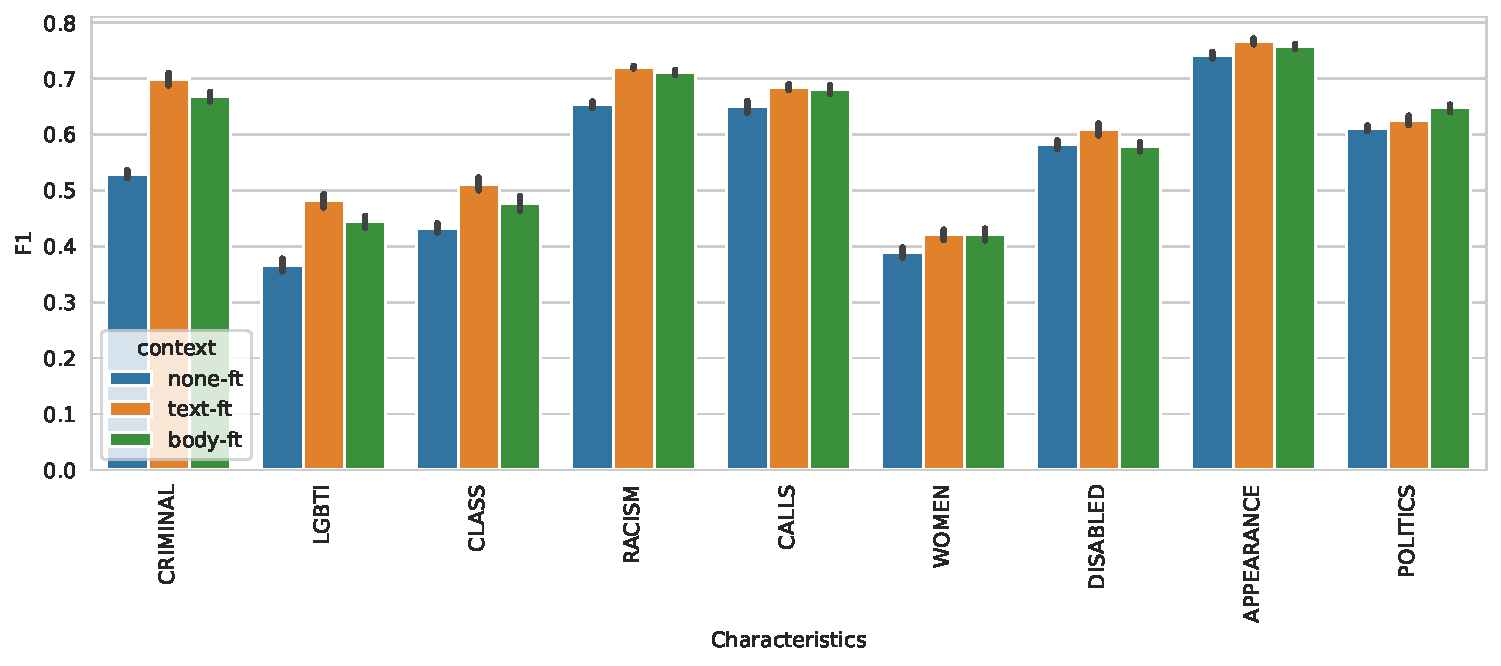
\includegraphics[width=\textwidth]{img/task_b_scores.pdf}
    \caption{Métrica F1 para cada característica de la tarea Task B. Las características están ordenadas de mayor a menor de acuerdo a la diferencia de performance entre el modelo sin contexto y el modelo contextualizado. }
    \label{fig:barplot_task_b_results}
\end{figure*}

La figura \ref{fig:barplot_task_b_results} muestra los resultados de las F1 por característica, esta vez ordenados de mayor a menor según el gap entre la performance contextualizada vs la no contextualizada, junto a sus intervalos de confianza 95\%, usando como modelos las versiones ajustadas al dominio. Todas las características obtienen una mejora estadísticamente significativa al correr un test Mann-Whitney U ($p \leq 0.005$, p valores ajustados por Benjamini-Hochberg\cite{benjamini1995controlling}). Las diferencias más sustanciales se dan en el caso de CRIMINAL ($+0.17$ F1 de diferencia), LGBTI ($+0.12$), CLASE ($+0.08$), y RACISMO (casi $+0.07$). Del otro lado, las características con menos mejora son APARIENCIA y POLITICA, algo esperable dado que el fenómeno tiene características poco dependientes del contexto (ver Apéndice \ref{app:manual_criterios_anotacion} para ejemplos).






\section{Análisis de error}

\section{Discusión}

Para analizar el impacto del contexto en la detección de discurso de odio, planteamos dos tareas de clasificación sobre el dataset construído en el capítulo \ref{chap:dataset_creation}: la tarea de detección binaria, donde respondemos si un comentario contiene discurso de odio; y una tarea de detección ``fina'', donde se debe mencionar la o las características protegidas ofendidas (si agrede a las mujeres, al colectivo LGBTI, si es racista, etc). En ambas tareas planteadas, propusimos clasificadores que consuman 3 tipos de entrada: el comentario sin contexto, el comentario con el contexto del tweet al que responden, y el comentario más el tweet al que responde y sumado el texto del artículo. Pudimos observar que el contexto parece dar una mejora moderada pero significativamente estadística en la tarea de detección del discurso de odio (alrededor de 3 puntos F1), y una mejora considerable en la tarea característica ofendida (alrededor de 6 puntos F1 medios).

Esto, en algún punto, indicaría que el contexto puede ser aprovechado para mejorar los algoritmos de detección de discurso de odio. Si bien este resultado podría estar en aparente contradicción con un trabajo reciente que no encontró ninguna mejora en el uso del contexto en la detección de toxicidad \cite{pavlopoulos2020toxicity}, se puede señalar que la detección del discurso de odio es una de las formas más complejas de comportamiento ``tóxico'' y, como tal, podría permitir que los clasificadores tengan más información para predecir si el texto dado es odioso o no. Otra razón detrás de este resultado es el dominio de nuestro conjunto de datos: mientras que \citet{pavlopoulos2020toxicity} usa el contexto conversacional, nosotros usamos el título y el cuerpo del artículo como contexto para los comentarios de los usuarios. Más recientemente, y como marcamos en la sección de trabajo previo, \citet{xenos-2021-context} ha observado que, restringiendo el análisis a un subconjunto de comentarios sensibles al contexto (ver \ref{sec:06_classification_previous} y \ref{sec:dataset_previous} para más información), la performance de los algoritmos de detección de toxicidad mejoran de manera significativa.

Algo que observamos es que la utilización de un contexto más largo como el artículo de la noticia no mejora la performance de nuestros clasificadores. Hay varias interpretaciones posibles de esto: en primer lugar, los humanos suelen contestar sin leer el artículo, con lo cual este resultado pareciera ser coherente con esta observación. Por otro lado, los humanos solemos tener acceso a un contexto mucho más rico, muchas veces equivalente a haber leído la nota, algo que nuestros clasificadores carecerían. Podría también esto ser atribuido al modelo pre-entrenado que usamos para codificar esto (BETO, la variante en español de BERT) que suele estar entrenada para textos más cortos (ver sección ZZZ para más información \todo{Escribir esto}). Teniendo esto en cuenta, realizamos el ajuste de dominio usando el contexto largo, pero aún así la performance del clasificador que consume este contexto ``largo'' se mantuvo por debajo del que usaba el contexto ``simple'' (sólo el tweet del artículo).

El análisis del error realizado demostró que, si bien el contexto pareciera mejorar la detección de discurso de odio, para muchas características protegidas se mantiene aún como una tarea difícil. Un caso ejemplificador de esto es la discriminación contra el colectivo LGBTI. Si bien el dataset recolectado no contiene demasiadas instancias de este fenómeno, en él puede verse que las agresiones contra este colectivo y sus miembros son sumamente sofisticadas, lejos de las agresiones meramente basadas en insultos u otras palabras ofensivas. Nuestros clasificadores, aún en sus mejores versiones (usando ajuste de dominio y contexto) obtuvieron una baja performance en la detección de este fenómeno (alrededor de $0.5$ F1 score) dando cuenta que es un problema no trivial y merece ser analizado más detenidamente debido a la complejidad de estos mensajes, que suelen reunir ironía, metáforas, y otros artilugios que hacen difícil su detección.

En el caso de la categoría mujer, inesperadamente, también obtuvimos una performance muy baja en la detección de agresiones misóginas. En el análisis de error, podemos observar que tenemos casos complejos de descifrar que fueron marcados por nuestros anotadores: por ejemplo, ataques ``velados'' a mujeres víctimas de violación (llamarlas mentirosas). \todo{Escribir un poco más sobre esto}

Algo que debe ser tenido en cuenta para matizar estos resultados es que utilizamos un amplio espectro de características protegidas. Incluso, la que más se beneficia del contexto es una que introdujimos ad-hoc para este experimento (discurso de odio contra criminales). En contrapeso, otras características ``no convencionales'' son poco beneficiadas por el contexto (como discurso de odio en base a la apariencia, opinión política y discapacidad).

Un resultado que también observamos es que pareciera ser que nuestros clasificadores mejoran su performance en un contexto de aprender cada característica por separado en vez de sólo aprender a distinguir la etiqueta binaria de discurso de odio.

Una limitación de aplicación de este resultado es que no siempre tenemos un contexto disponible para un texto dado. Incluso si podemos encontrarlo, a veces este contexto puede no ser en forma de artículo de noticias, sino como un hilo de conversación o incluso de alguna otra forma (¿una base de conocimiento?). Teniendo en cuenta alguna de las consideraciones hechas en esta discusión, una posible línea de investigación seria la de incorporar distintos tipos de contexto, desde más mensajes en el hilo de la conversación como así también conocimiento estructurado \todo{Agregar alguna cita, quizás de knowledge infusion}

\section{Conclusiones}

En este capítulo hemos explorado diversos experimentos para responder nuestra pregunta original: ¿Puede el contexto de un mensaje ser usado para mejorar la detección de discurso de odio? Utilizando el dataset especialmente construído a tal fin en el capítulo anterior y planteando tareas de clasificación sobre éste, obtuvimos evidencia que indicaría que, para el dominio específico de los comentarios en redes sociales sobre noticias periodísticas, el contexto mejora de manera estadísticamente significativa la performance de los algoritmos de detección.